% Options for packages loaded elsewhere
\PassOptionsToPackage{unicode}{hyperref}
\PassOptionsToPackage{hyphens}{url}
%
\documentclass[
]{article}
\usepackage{amsmath,amssymb}
\usepackage{lmodern}
\usepackage{iftex}
\ifPDFTeX
  \usepackage[T1]{fontenc}
  \usepackage[utf8]{inputenc}
  \usepackage{textcomp} % provide euro and other symbols
\else % if luatex or xetex
  \usepackage{unicode-math}
  \defaultfontfeatures{Scale=MatchLowercase}
  \defaultfontfeatures[\rmfamily]{Ligatures=TeX,Scale=1}
\fi
% Use upquote if available, for straight quotes in verbatim environments
\IfFileExists{upquote.sty}{\usepackage{upquote}}{}
\IfFileExists{microtype.sty}{% use microtype if available
  \usepackage[]{microtype}
  \UseMicrotypeSet[protrusion]{basicmath} % disable protrusion for tt fonts
}{}
\makeatletter
\@ifundefined{KOMAClassName}{% if non-KOMA class
  \IfFileExists{parskip.sty}{%
    \usepackage{parskip}
  }{% else
    \setlength{\parindent}{0pt}
    \setlength{\parskip}{6pt plus 2pt minus 1pt}}
}{% if KOMA class
  \KOMAoptions{parskip=half}}
\makeatother
\usepackage{xcolor}
\usepackage[margin=1in]{geometry}
\usepackage{graphicx}
\makeatletter
\def\maxwidth{\ifdim\Gin@nat@width>\linewidth\linewidth\else\Gin@nat@width\fi}
\def\maxheight{\ifdim\Gin@nat@height>\textheight\textheight\else\Gin@nat@height\fi}
\makeatother
% Scale images if necessary, so that they will not overflow the page
% margins by default, and it is still possible to overwrite the defaults
% using explicit options in \includegraphics[width, height, ...]{}
\setkeys{Gin}{width=\maxwidth,height=\maxheight,keepaspectratio}
% Set default figure placement to htbp
\makeatletter
\def\fps@figure{htbp}
\makeatother
\setlength{\emergencystretch}{3em} % prevent overfull lines
\providecommand{\tightlist}{%
  \setlength{\itemsep}{0pt}\setlength{\parskip}{0pt}}
\setcounter{secnumdepth}{-\maxdimen} % remove section numbering
\usepackage{booktabs}
\usepackage{longtable}
\usepackage{array}
\usepackage{multirow}
\usepackage{wrapfig}
\usepackage{float}
\usepackage{colortbl}
\usepackage{pdflscape}
\usepackage{tabu}
\usepackage{threeparttable}
\usepackage{threeparttablex}
\usepackage[normalem]{ulem}
\usepackage{makecell}
\usepackage{xcolor}
\ifLuaTeX
  \usepackage{selnolig}  % disable illegal ligatures
\fi
\IfFileExists{bookmark.sty}{\usepackage{bookmark}}{\usepackage{hyperref}}
\IfFileExists{xurl.sty}{\usepackage{xurl}}{} % add URL line breaks if available
\urlstyle{same} % disable monospaced font for URLs
\hypersetup{
  pdftitle={Análises Danielle},
  pdfauthor={Samuel Martins de Medeiros},
  hidelinks,
  pdfcreator={LaTeX via pandoc}}

\title{Análises Danielle}
\author{Samuel Martins de Medeiros}
\date{}

\begin{document}
\maketitle

\hypertarget{panorama-geral}{%
\section{Panorama Geral}\label{panorama-geral}}

\hypertarget{avaliauxe7uxe3o-geral-de-mortalidade}{%
\subsection{Avaliação geral de
mortalidade}\label{avaliauxe7uxe3o-geral-de-mortalidade}}

Tendo em vista a disposição dos dados das gestantes e das não gestantes,
será realizada uma análise para ambos os grupos. Em primeiro lugar, será
feita uma avaliação geral da frequência absoluta, a fim de verificar a
categoria com maior concentração. Na Tabela 1, é possível observar a
frequência total e relativa por tipo de mortalidade. Observa-se que a
quantidade de observações está predominantemente nas classificações de
Homicídio e Acidente automobilístico, mantendo esse padrão para ambos os
grupos analisados. Vemos um valor considerável apenas na categoria de
suicídio fora as já citadas. Além disso, percebe-se que o comportamento
difere entre o grupo de gestantes e o grupo de não gestantes. No grupo
gestante, a variável Acidente Automobilístico apresenta uma porcentagem
superior à de Homicídios, enquanto no grupo de não gestantes ocorre o
contrário.

\begin{table}

\caption{\label{tab:unnamed-chunk-1}Tabela de frequências por tipo de mortalidade}
\centering
\begin{tabular}[t]{l|r|r|r|r}
\hline
  & n (Gest.) & \% (Gest.) & n (Não
                 ) & \% (Não)\\
\hline
Acidente automobilísticos & 1023 & 31.1 & 44761 & 34.7\\
\hline
Acidente Envenenamento acidental & 147 & 4.5 & 2828 & 2.2\\
\hline
Acidente Eventos ambientais & 48 & 1.5 & 1954 & 1.5\\
\hline
Acidente Quedas/ afogamento/inalação/ corrente elétrica & 171 & 5.2 & 10389 & 8.1\\
\hline
Homicídio & 1308 & 39.7 & 37567 & 29.1\\
\hline
Outro & 214 & 6.5 & 12139 & 9.4\\
\hline
Suicídio & 383 & 11.6 & 19261 & 14.9\\
\hline
Total & 3294 & 100.0 & 128899 & 100.0\\
\hline
\end{tabular}
\end{table}

Uma outra forma de verificar as afirmações citadas, apresentando os
mesmos resultados, é por meio da Figura 1, que fornece um apoio visual.
Os dados são apresentados da seguinte forma:

\begin{itemize}
\item
  X1: Acidente automobilístico;
\item
  X2: Acidente por envenenamento acidental;
\item
  X3: Acidente por eventos ambientais;
\item
  X4: Acidente por quedas/afogamento/inalação/corrente elétrica;
\item
  X5: Homicídio;
\item
  X6: Outro;
\item
  X7: Suicídio.
\end{itemize}

Essa definição será adotada novamente ao longo do relatório, quando
necessário, para facilitar a referência às legendas dos gráficos e
tabelas.

\begin{figure}
\centering
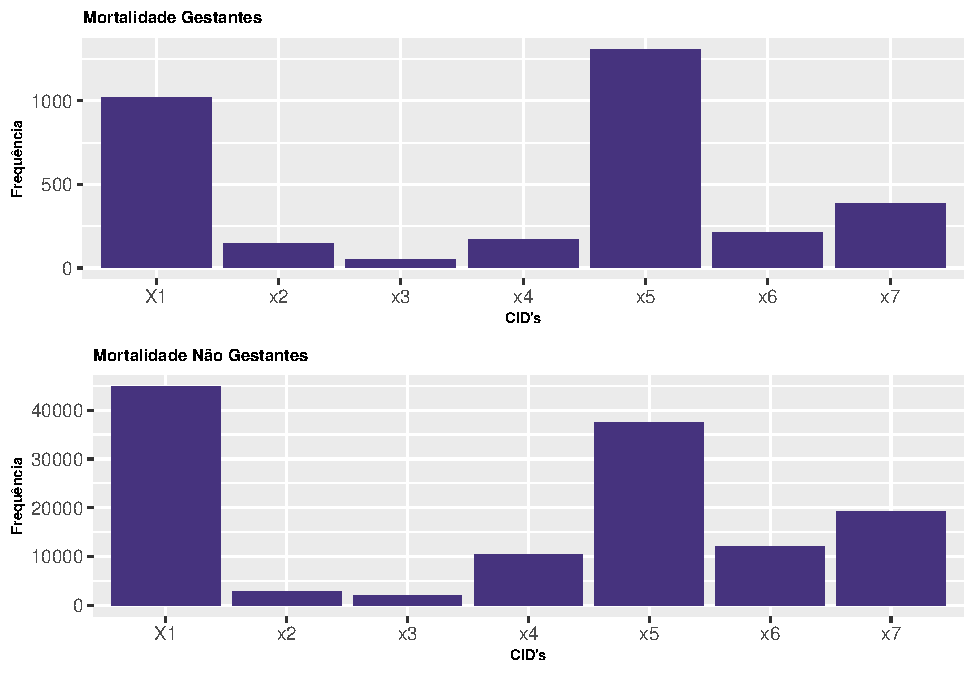
\includegraphics{RelatorioV01_files/figure-latex/unnamed-chunk-2-1.pdf}
\caption{Frequência por CID}
\end{figure}

Outro objetivo da investigação é analisar a distribuição ao longo dos
anos. Conforme mostrado na Figura 2, observa-se um comportamento
diferente nos anos de 2017 a 2019 para o grupo de gestantes. Enquanto as
outras causas CID apresentam uma diminuição na frequência, é possível
notar um leve aumento no caso de suicídio. Também é evidente uma
estabilidade de 2019 a 2020, em comparação com os demais anos. Em
relação ao homicídio, há um pico em 2017, com um valor de 161,
correspondendo a 12,30\% dos dados totais de homicídio e a 46,80\% dos
dados totais de morte em 2017.

Já para o grupo de não gestantes, observa-se um comportamento diferente
nos anos mencionados anteriormente, com uma queda geral, incluindo na
variável homicídio, e uma estabilidade geral. Isso também pode ser
atribuído à quantidade absoluta de observações. É visível que a
quantidade de mortes em geral para esse grupo tem diminuído de forma
pequena ao longo dos anos.

\begin{figure}
\centering
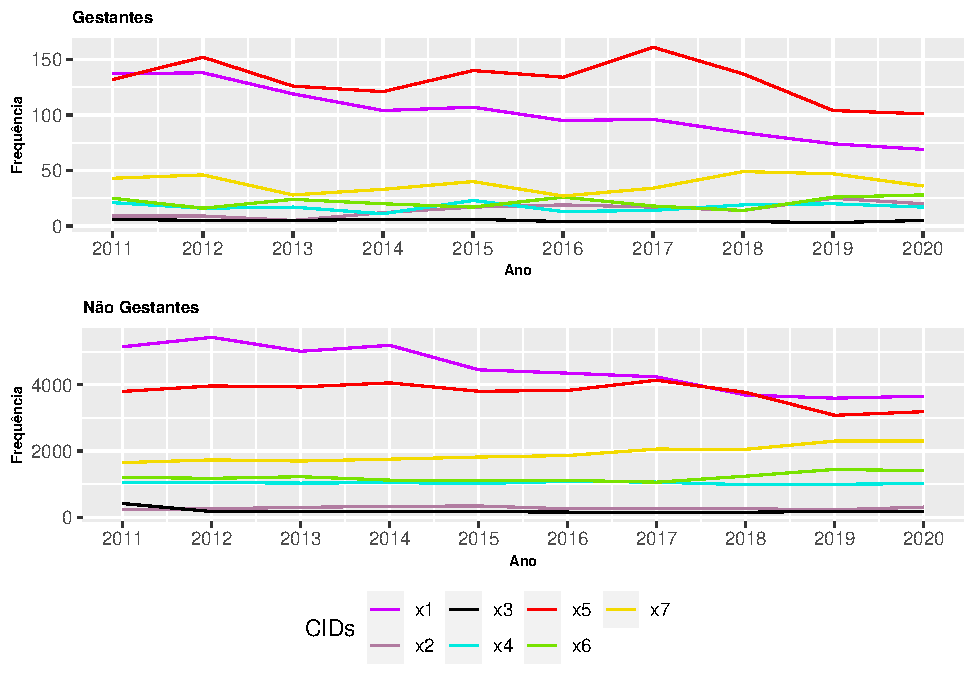
\includegraphics{RelatorioV01_files/figure-latex/unnamed-chunk-3-1.pdf}
\caption{Séries Temporáis por CID}
\end{figure}

\hypertarget{variuxe1veis-de-caracterizauxe7uxe3o}{%
\subsection{Variáveis de
Caracterização}\label{variuxe1veis-de-caracterizauxe7uxe3o}}

Continuando com a avaliação das variáveis de caracterização do objeto de
estudo, será feita uma comparação das CID's por sexo, raça, escolaridade
e estado civil, nessa ordem, apresentando tabelas de frequência e
proporções para ambos, com as devidas observações importantes
identificadas, além de uma avaliação do número de mortes totais por ano
para as categorias disponíveis de cada uma das variáveis.

\hypertarget{sexo}{%
\subsubsection{Sexo}\label{sexo}}

Neste tópico, é possível identificar certas inconsistências dentro do
próprio banco de dados, como mostrado na Tabela 2. Para o grupo de
gestantes, há uma observação com o sexo marcado como masculino, o que é
inadequado para esse grupo específico. Para a variável sexo, como temos
apenas 2 observações que diferem do valor esperado da comparação geral,
não serão realizadas as demais análises (tabelas de frequência absoluta
e gráficos por ano), uma vez que os resultados seriam os mesmos, com
exceção das duas observações mencionadas.

\begin{table}

\caption{\label{tab:unnamed-chunk-4}Tabela de frequências (Gestantes)}
\centering
\begin{tabular}[t]{l|r|r|r}
\hline
  & Feminino & Ignorado & Masculino\\
\hline
Acidente automobilísticos & 1023 & 0 & 0\\
\hline
Acidente Envenenamento acidental & 147 & 0 & 0\\
\hline
Acidente Eventos ambientais & 48 & 0 & 0\\
\hline
Acidente Quedas/ afogamento/inalação/ corrente elétrica & 170 & 1 & 0\\
\hline
Homicídio & 1308 & 0 & 0\\
\hline
Outro & 212 & 1 & 1\\
\hline
Suicídio & 383 & 0 & 0\\
\hline
\end{tabular}
\end{table}

\hypertarget{rauxe7a}{%
\subsubsection{Raça}\label{rauxe7a}}

Para a variável Raça, temos as seguintes possibilidades: Branca, Parda,
Preta, Ignorado, Indígena e Amarela. Ao analisar os valores absolutos
para a população branca e parda, tanto de forma geral quanto por grupo,
observa-se uma diferença significativa entre a terceira maior raça e a
segunda maior raça. A diferença é grande, com 53.707 para a raça parda e
8.085 para a raça branca, quando somadas as observações dos grupos, como
mostra a Tabela 3.

Inicialmente, para o grupo de gestantes, considerando apenas a tabela de
CID x Raça (Tabela 4), percebe-se um comportamento semelhante para todas
as raças, exceto para a raça preta, que apresenta um valor um pouco mais
elevado em proporção para Acidente por envenenamento acidental em
comparação com Acidente por quedas/afogamento/inalação/corrente
elétrica. Além disso, há uma concentração de 50\% dos valores em
Homicídio para a raça preta.

Já para o grupo de não gestantes, o comportamento segue de forma
diferente, com valores maiores para acidentes automobilísticos, como
mostra a Tabela 5, e uma queda na proporção de homicídios.

\begin{table}

\caption{\label{tab:unnamed-chunk-5}Tabela de frequências por Raça}
\centering
\begin{tabular}[t]{l|r|r|r|r|r|r}
\hline
  & Amarela & Branca & Ignorado & Indígena & Parda & Preta\\
\hline
Gestante & 2 & 1201 & 82 & 37 & 1718 & 254\\
\hline
Não & 294 & 52505 & 3856 & 804 & 63609 & 7831\\
\hline
total & 296 & 53706 & 3938 & 841 & 65327 & 8085\\
\hline
\end{tabular}
\end{table}

\begin{table}

\caption{\label{tab:unnamed-chunk-5}Tabela de proporção de CIDs por Raça (Gestantes)}
\centering
\begin{tabular}[t]{l|r|r|r|r|r|r}
\hline
  & Amarela & Branca & Ignorado & Indígena & Parda & Preta\\
\hline
x1 & 0.0 & 0.40 & 0.18 & 0.19 & 0.28 & 0.15\\
\hline
x2 & 0.0 & 0.04 & 0.04 & 0.00 & 0.04 & 0.07\\
\hline
x3 & 0.0 & 0.01 & 0.02 & 0.08 & 0.02 & 0.01\\
\hline
x4 & 0.0 & 0.04 & 0.07 & 0.03 & 0.05 & 0.07\\
\hline
x5 & 0.5 & 0.32 & 0.38 & 0.43 & 0.43 & 0.52\\
\hline
x6 & 0.0 & 0.06 & 0.15 & 0.11 & 0.06 & 0.07\\
\hline
x7 & 0.5 & 0.12 & 0.16 & 0.16 & 0.11 & 0.11\\
\hline
\end{tabular}
\end{table}

\begin{table}

\caption{\label{tab:unnamed-chunk-5}Tabela de proporção de CIDs por Raça  (Não)}
\centering
\begin{tabular}[t]{l|r|r|r|r|r|r}
\hline
  & Amarela & Branca & Ignorado & Indígena & Parda & Preta\\
\hline
x1 & 0.31 & 0.39 & 0.31 & 0.18 & 0.32 & 0.25\\
\hline
x2 & 0.02 & 0.02 & 0.02 & 0.01 & 0.02 & 0.04\\
\hline
x3 & 0.01 & 0.02 & 0.01 & 0.05 & 0.01 & 0.02\\
\hline
x4 & 0.08 & 0.07 & 0.08 & 0.10 & 0.08 & 0.10\\
\hline
x5 & 0.20 & 0.21 & 0.33 & 0.23 & 0.35 & 0.34\\
\hline
x6 & 0.12 & 0.09 & 0.12 & 0.07 & 0.09 & 0.12\\
\hline
x7 & 0.26 & 0.19 & 0.12 & 0.36 & 0.12 & 0.12\\
\hline
\end{tabular}
\end{table}

De forma geral, conforme mostrado na Figura 3, é possível observar uma
maior estabilidade para as raças Preta, Ignorado e Indígena ao longo do
tempo. A variável raça Branca apresenta uma oscilação maior, como pode
ser observado de forma mais acentuada no grupo de gestantes, com um
aumento significativo de 2014 para 2015 e uma queda considerável de 2019
para 2020. A mesma variação pode ser observada para a raça Parda, com um
aumento acentuado de 2016 para 2017 em ambos os grupos. A partir de
2015, ambos os grupos parecem seguir um comportamento semelhante,
enquanto nos anos anteriores é possível observar uma queda significativa
de 2012 para 2013 no grupo de gestantes, enquanto no grupo de não
gestantes há uma maior estabilidade.

\begin{figure}
\centering
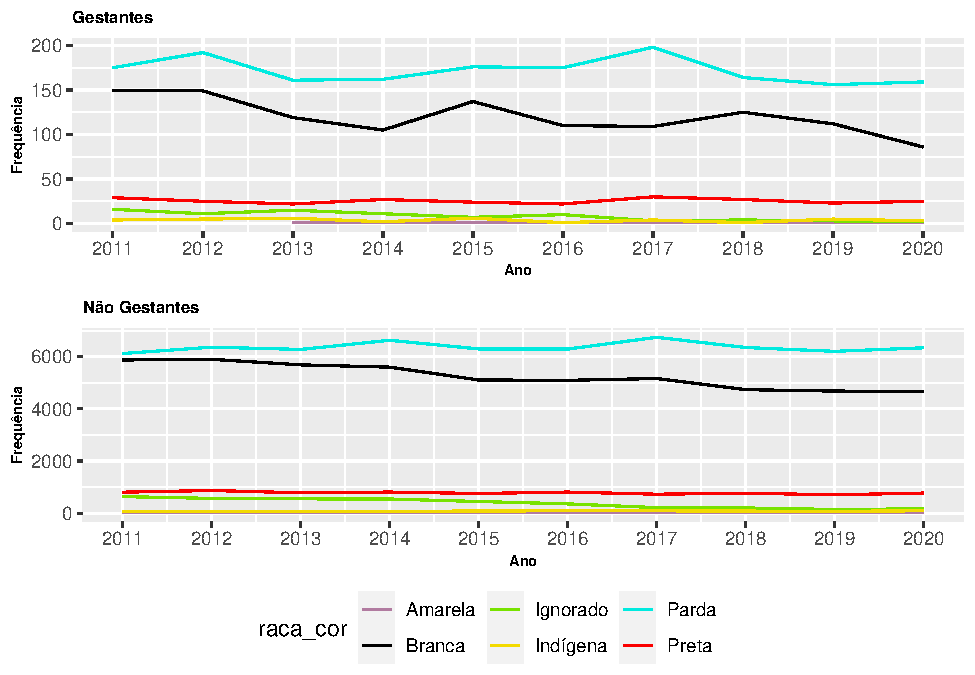
\includegraphics{RelatorioV01_files/figure-latex/unnamed-chunk-6-1.pdf}
\caption{Séries Temporáis por Raça}
\end{figure}

Considerando as opções de escolaridade: Fundamental I, Fundamental II,
Ignorado, Médio, Sem escolaridade, Superior Completo e Superior
Incompleto, observamos um comportamento semelhante nos dois grupos, com
uma predominância da escolaridade no nível Fundamental II, seguida pelo
nível Médio. A diferença entre os dois níveis é baixa, conforme visto na
Tabela 6.

Um fato interessante é evidenciado tanto na Tabela 7 quanto na Tabela 8.
Conforme o nível de escolaridade aumenta, há uma redução na proporção de
homicídios. Tomando o exemplo do grupo de gestantes, observa-se que 48\%
dos homicídios ocorrem em indivíduos com escolaridade no nível
Fundamental II, enquanto apenas 17\% ocorrem em indivíduos com Ensino
Superior Completo. Essa porcentagem, que não é observada em homicídios,
é distribuída entre as categorias de Suicídio e Acidente automobilístico
para pessoas com maior nível de escolaridade.

\begin{table}

\caption{\label{tab:unnamed-chunk-7}Tabela de frequências por Escolaridade}
\centering
\begin{tabular}[t]{l|r|r|r|r|r|r|r}
\hline
  & Fund. I & Fund. II & Ignorado & Médio & Sem escolaridade & Superior Compl. & Superior Incom.\\
\hline
Gestante & 400 & 1005 & 345 & 663 & 41 & 151 & 73\\
\hline
Não & 17473 & 31502 & 15147 & 25766 & 3442 & 7660 & 4191\\
\hline
total & 17873 & 32507 & 15492 & 26429 & 3483 & 7811 & 4264\\
\hline
\end{tabular}
\end{table}

\begin{table}

\caption{\label{tab:unnamed-chunk-7}Tabela de proporção de CIDs por Escolaridade (Gestantes)}
\centering
\begin{tabular}[t]{l|r|r|r|r|r|r|r}
\hline
  & Fund. I & Fund. II & Ignorado & Médio & Sem escolaridade & Superior Compl. & Superior Incom.\\
\hline
x1 & 0.25 & 0.24 & 0.36 & 0.35 & 0.37 & 0.44 & 0.53\\
\hline
x2 & 0.07 & 0.07 & 0.01 & 0.04 & 0.00 & 0.03 & 0.00\\
\hline
x3 & 0.01 & 0.02 & 0.01 & 0.02 & 0.00 & 0.01 & 0.01\\
\hline
x4 & 0.07 & 0.04 & 0.04 & 0.05 & 0.07 & 0.06 & 0.01\\
\hline
x5 & 0.44 & 0.48 & 0.42 & 0.34 & 0.39 & 0.17 & 0.23\\
\hline
x6 & 0.06 & 0.06 & 0.07 & 0.07 & 0.12 & 0.08 & 0.03\\
\hline
x7 & 0.09 & 0.10 & 0.10 & 0.14 & 0.05 & 0.22 & 0.18\\
\hline
\end{tabular}
\end{table}

\begin{table}

\caption{\label{tab:unnamed-chunk-7}Tabela de proporção de CIDs por Escolaridade  (Não)}
\centering
\begin{tabular}[t]{l|r|r|r|r|r|r|r}
\hline
  & Fund. I & Fund. II & Ignorado & Médio & Sem escolaridade & Superior Compl. & Superior Incom.\\
\hline
x1 & 0.29 & 0.30 & 0.35 & 0.40 & 0.24 & 0.43 & 0.45\\
\hline
x2 & 0.02 & 0.03 & 0.01 & 0.02 & 0.02 & 0.02 & 0.02\\
\hline
x3 & 0.02 & 0.01 & 0.01 & 0.01 & 0.03 & 0.01 & 0.01\\
\hline
x4 & 0.10 & 0.08 & 0.08 & 0.07 & 0.22 & 0.06 & 0.05\\
\hline
x5 & 0.34 & 0.36 & 0.29 & 0.24 & 0.24 & 0.13 & 0.15\\
\hline
x6 & 0.10 & 0.09 & 0.10 & 0.10 & 0.14 & 0.10 & 0.10\\
\hline
x7 & 0.13 & 0.13 & 0.16 & 0.17 & 0.11 & 0.24 & 0.22\\
\hline
\end{tabular}
\end{table}

Com relação à mortalidade por escolaridade analisada ao longo dos anos
(Figura 4), vamos reduzir os comentários apenas ao grupo de gestantes,
pois para o grupo complementar as séries indicam uma maior constância.

No que diz respeito ao grupo de gestantes, observa-se que o número de
mortes de 2013 a 2015 apresentou um aumento considerável para o grupo de
Ensino Médio, com um pico que não é identificado nas outras categorias.
Além disso, há um aumento significativo de 2018 a 2020, que é observado
apenas nessa categoria. As variáveis de Ensino Superior Completo, Ensino
Superior Incompleto e Sem escolaridade parecem ter um comportamento
equilibrado e constante ao longo da janela de tempo total analisada.

\begin{figure}
\centering
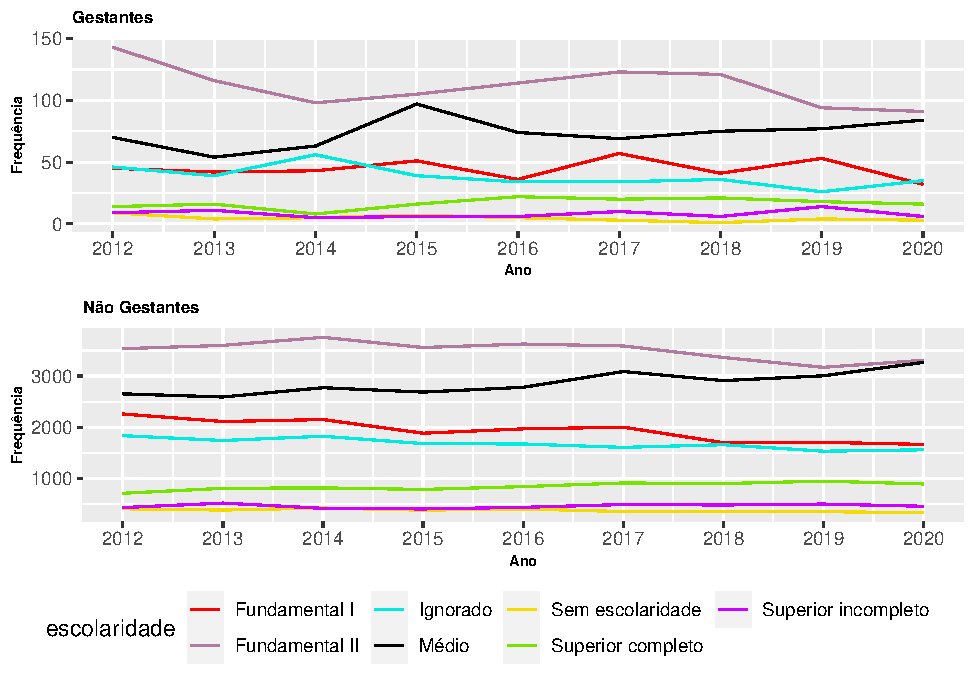
\includegraphics{RelatorioV01_files/figure-latex/unnamed-chunk-8-1.pdf}
\caption{Séries Temporáis por Escolaridade}
\end{figure}

\hypertarget{estado-civil}{%
\subsubsection{Estado Civil}\label{estado-civil}}

Ao comparar os resultados para as categorias: Casado, Solteiro,
Ignorado, Separado Judic./Divorciado e Viúvo, observamos um número
significativamente maior de indivíduos solteiros, seguido pelos casados,
conforme mostrado na Tabela 9.

No grupo de gestantes, é possível notar uma taxa de homicídios muito
maior entre os indivíduos solteiros em comparação com o outro grupo,
como evidenciado na Tabela 10. Além disso, há um valor elevado de
acidentes automobilísticos entre a categoria Casado. Esse mesmo
comportamento, em relação à categoria Casado, é observado no grupo de
não gestantes, conforme mostrado na Tabela 11, apresentando um
comportamento mais equilibrado entre as demais categorias de CID's.

\begin{table}

\caption{\label{tab:unnamed-chunk-9}Tabela de frequências por Estado Civil}
\centering
\begin{tabular}[t]{l|r|r|r|r|r}
\hline
  & Casado & Ignorado & Separado Judic./Divorciado & Solteiro & Viúvo\\
\hline
Gestante & 476 & 601 & 64 & 2137 & 16\\
\hline
Não & 24281 & 17493 & 7047 & 77522 & 2556\\
\hline
total & 24757 & 18094 & 7111 & 79659 & 2572\\
\hline
\end{tabular}
\end{table}

\begin{table}

\caption{\label{tab:unnamed-chunk-9}Tabela de proporção de CIDs por Estado Civil (Gestantes)}
\centering
\begin{tabular}[t]{l|r|r|r|r|r}
\hline
  & Casado & Ignorado & Separado Judic./Divorciado & Solteiro & Viúvo\\
\hline
x1 & 0.51 & 0.35 & 0.31 & 0.26 & 0.25\\
\hline
x2 & 0.03 & 0.02 & 0.06 & 0.06 & 0.00\\
\hline
x3 & 0.01 & 0.02 & 0.02 & 0.02 & 0.00\\
\hline
x4 & 0.06 & 0.07 & 0.06 & 0.04 & 0.19\\
\hline
x5 & 0.18 & 0.38 & 0.28 & 0.45 & 0.31\\
\hline
x6 & 0.07 & 0.06 & 0.14 & 0.06 & 0.12\\
\hline
x7 & 0.14 & 0.11 & 0.12 & 0.11 & 0.12\\
\hline
\end{tabular}
\end{table}

\begin{table}

\caption{\label{tab:unnamed-chunk-9}Tabela de proporção de CIDs por Estado Civil  (Não)}
\centering
\begin{tabular}[t]{l|r|r|r|r|r}
\hline
  & Casado & Ignorado & Separado Judic./Divorciado & Solteiro & Viúvo\\
\hline
x1 & 0.42 & 0.35 & 0.35 & 0.33 & 0.38\\
\hline
x2 & 0.02 & 0.02 & 0.02 & 0.02 & 0.03\\
\hline
x3 & 0.02 & 0.02 & 0.02 & 0.01 & 0.02\\
\hline
x4 & 0.08 & 0.08 & 0.07 & 0.08 & 0.11\\
\hline
x5 & 0.18 & 0.32 & 0.22 & 0.33 & 0.21\\
\hline
x6 & 0.11 & 0.09 & 0.11 & 0.09 & 0.12\\
\hline
x7 & 0.18 & 0.14 & 0.23 & 0.14 & 0.15\\
\hline
\end{tabular}
\end{table}

Podemos observar na Figura 5 a hipótese já mencionada sobre o número
elevado de mortalidade para a categoria Solteiro, além de ser a
categoria que apresenta uma maior instabilidade ao longo dos anos,
especialmente entre 2012 e 2015. De forma geral, não parece apresentar
nenhuma outra variabilidade considerável.

\begin{figure}
\centering
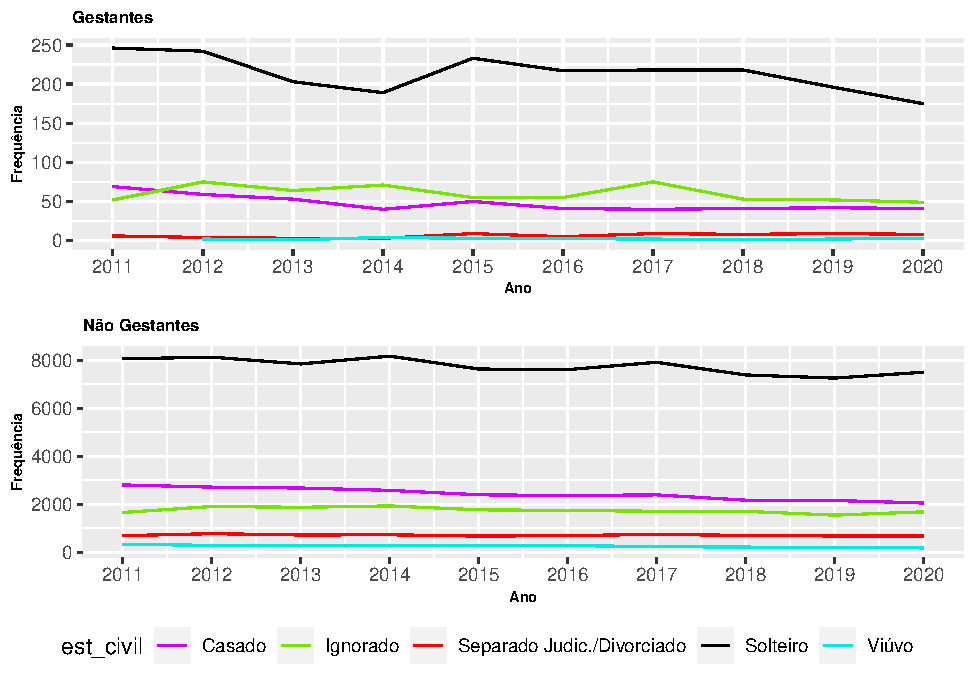
\includegraphics{RelatorioV01_files/figure-latex/unnamed-chunk-10-1.pdf}
\caption{Séries Temporáis por Estado Civil}
\end{figure}

\hypertarget{variuxe1veis-de-regionalizauxe7uxe3o}{%
\subsection{Variáveis de
Regionalização}\label{variuxe1veis-de-regionalizauxe7uxe3o}}

A fim de identificar padrões no perfil de gestantes e não gestantes em
relação ao tipo de mortalidade, foi realizada uma análise de
caracterização considerando a regionalização dos indivíduos por UF
(Unidade Federativa) de residência e ocorrência. Devido ao grande número
de UF's presentes, serão apresentados resultados apenas para os 10
estados com o maior número de ocorrências registradas.

\hypertarget{ufs-de-residuxeancia}{%
\subsubsection{UF's de residência}\label{ufs-de-residuxeancia}}

Conforme apresentado na Tabela 12, os três estados com o maior número de
mortalidade são: São Paulo, Minas Gerais e Rio de Janeiro. Esses estados
estão localizados na região Sudeste, que também é a região mais populosa
do Brasil.

\begin{table}

\caption{\label{tab:unnamed-chunk-11}Tabela de frequências por UF de residência}
\centering
\begin{tabular}[t]{l|r|r|r|r|r|r|r|r|r|r}
\hline
  & BA & CE & GO & MG & PA & PE & PR & RJ & RS & SP\\
\hline
Gestante & 192 & 167 & 155 & 278 & 121 & 134 & 282 & 303 & 182 & 496\\
\hline
Não & 9616 & 6566 & 5856 & 13065 & 5460 & 6226 & 8058 & 10137 & 7171 & 20608\\
\hline
total & 9808 & 6733 & 6011 & 13343 & 5581 & 6360 & 8340 & 10440 & 7353 & 21104\\
\hline
\end{tabular}
\end{table}

\begin{table}

\caption{\label{tab:unnamed-chunk-11}Tabela de proporção de CIDs por UF de residência (Gestantes)}
\centering
\begin{tabular}[t]{l|r|r|r|r|r|r|r|r|r|r}
\hline
  & BA & CE & GO & MG & PA & PE & PR & RJ & RS & SP\\
\hline
x1 & 0.25 & 0.22 & 0.41 & 0.30 & 0.33 & 0.28 & 0.43 & 0.17 & 0.29 & 0.32\\
\hline
x2 & 0.01 & 0.01 & 0.01 & 0.03 & 0.03 & 0.00 & 0.01 & 0.21 & 0.01 & 0.09\\
\hline
x3 & 0.02 & 0.01 & 0.01 & 0.01 & 0.02 & 0.00 & 0.01 & 0.04 & 0.00 & 0.02\\
\hline
x4 & 0.08 & 0.04 & 0.03 & 0.05 & 0.10 & 0.08 & 0.02 & 0.06 & 0.03 & 0.04\\
\hline
x5 & 0.44 & 0.50 & 0.44 & 0.41 & 0.36 & 0.49 & 0.43 & 0.34 & 0.53 & 0.29\\
\hline
x6 & 0.13 & 0.08 & 0.04 & 0.08 & 0.05 & 0.08 & 0.02 & 0.08 & 0.02 & 0.10\\
\hline
x7 & 0.08 & 0.14 & 0.06 & 0.12 & 0.11 & 0.07 & 0.08 & 0.11 & 0.13 & 0.14\\
\hline
\end{tabular}
\end{table}

\begin{table}

\caption{\label{tab:unnamed-chunk-11}Tabela de proporção de CIDs por UF de residência  (Não)}
\centering
\begin{tabular}[t]{l|r|r|r|r|r|r|r|r|r|r}
\hline
  & BA & CE & GO & MG & PA & PE & PR & RJ & RS & SP\\
\hline
x1 & 0.27 & 0.29 & 0.40 & 0.34 & 0.34 & 0.29 & 0.44 & 0.27 & 0.33 & 0.35\\
\hline
x2 & 0.02 & 0.01 & 0.01 & 0.02 & 0.01 & 0.02 & 0.01 & 0.09 & 0.01 & 0.03\\
\hline
x3 & 0.01 & 0.01 & 0.01 & 0.02 & 0.01 & 0.01 & 0.01 & 0.05 & 0.01 & 0.02\\
\hline
x4 & 0.09 & 0.07 & 0.06 & 0.08 & 0.09 & 0.09 & 0.06 & 0.11 & 0.07 & 0.09\\
\hline
x5 & 0.38 & 0.38 & 0.34 & 0.25 & 0.40 & 0.34 & 0.26 & 0.28 & 0.28 & 0.20\\
\hline
x6 & 0.15 & 0.12 & 0.04 & 0.12 & 0.07 & 0.14 & 0.07 & 0.10 & 0.07 & 0.14\\
\hline
x7 & 0.08 & 0.13 & 0.14 & 0.18 & 0.09 & 0.10 & 0.15 & 0.10 & 0.23 & 0.18\\
\hline
\end{tabular}
\end{table}

Vale destacar, de acordo com a Tabela 13 e 14, a concentração de
acidentes automobilísticos em Goiás (GO) e Paraná (PR), bem como a taxa
de homicídios apresentada nos estados do Nordeste, como Ceará (CE),
Pernambuco (PE) e Bahia (BA), e nos estados do Sul, como Santa Catarina
(SC) e Paraná (PR).

Para os estados mencionados como tendo o maior índice total, São Paulo
(SP) e Minas Gerais (MG), observa-se uma distribuição relativamente
equilibrada entre acidentes automobilísticos e homicídios. Já para o Rio
de Janeiro (RJ), são observados valores um pouco mais acentuados em
acidentes por envenenamento acidental no grupo de gestantes, mas esse
padrão não se repete no grupo de não gestantes.

\begin{figure}
\centering
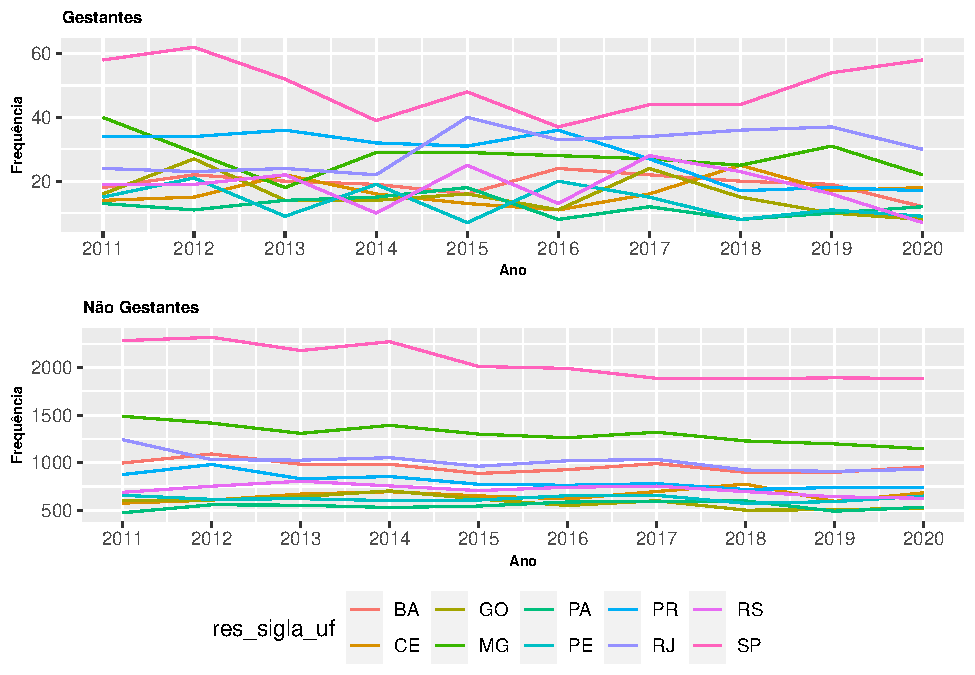
\includegraphics{RelatorioV01_files/figure-latex/unnamed-chunk-12-1.pdf}
\caption{Séries Temporáis por UF de Residência}
\end{figure}

No que diz respeito à Figura 6, podemos observar um equilíbrio no grupo
de não gestantes, com uma leve queda no caso da Bahia (BA). No entanto,
o mesmo padrão não pode ser evidenciado no grupo de gestantes, onde é
observada uma variabilidade maior na maioria dos estados, especialmente
em São Paulo (SP) e Paraná (PR). Para São Paulo, que apresenta a maior
variabilidade no grupo de gestantes, podemos observar uma redução
acentuada de 2012 a 2014, seguida por um crescimento significativo nos
períodos seguintes, enquanto no estado do Paraná ocorre um comportamento
mais aproximado do constante até o ano de 2016, onde apresenta um queda
para 2020 significativa. Ao que tudo indica todos os estados, com
excessão de São Paulo, parecem estar apresentando uma tendência a
redução de 2019 para 2020.

\hypertarget{ufs-de-ocorruxeancia}{%
\subsubsection{UF's de Ocorrência}\label{ufs-de-ocorruxeancia}}

Conforme observado na Tabela 15, o padrão é semelhante ao das UF's de
residência, com os estados de São Paulo (SP), Minas Gerais (MG) e Rio de
Janeiro (RJ) concentrando a maior parte das ocorrências.

De forma geral, o comportamento das UF's de ocorrência segue o padrão
apresentado nas UF's de residência (Tabelas 16 e 17), tanto para as
CID's de homicídio quanto para acidentes automobilísticos, como
mencionado anteriormente.

\begin{verbatim}
## Time differences in days
##    [1]  7886 12303 12602  7885 15574  7374  6351  7000  5565  6343  6381  9686
##   [13] 12408  7476  8925  8026 11918 11345  9661  8017 10634  7589 12849  7564
##   [25]  7590 19574  6969  3627 11757  8151  7093  8804  8830  9542 10905 16783
##   [37]  7802 13622  6858 11191  8706 18615 11051  5775  9264  5640  4795  8503
##   [49]  7490 15104 11487  7057 13838 15901  5747 14082 10393  8393  6678  5428
##   [61]  9571  6392 20569  9625 10435  6843  8660 11400  9671  7475  9191  6300
##   [73] 10075 12527  9355  8884 10762 20805  9684 11018 18056 13356 11189  6621
##   [85]  7847  9065 12500  6359  7917  7699 14574  6746 10520  6793 18852  6691
##   [97] 10371  9667 10568 12053  4547  6523  5990  7381 11167 18347 11614  7190
##  [109]  8903  6471 10764  7139 11124  4375  6504  6682 19693 12509  6546  6195
##  [121]  8296 13522 12564  8156 19576 10255  6754 13944 12597  6478  7803  5237
##  [133]  6529 10031  7953  7332  9112  7580 10827  6766  7513  6137 13559  6838
##  [145]  6466 13657 11469    NA  5034  9458 12861  7386  6110  8208  6676  8721
##  [157]  9498  7041  8381  8864 13786  5867  6444  6147  8671 12230 12777 11611
##  [169]  6766 13886 19918  8189 11772  8711  7466  9553 13749  8387  5977 17198
##  [181] 13745 14342 10313  6556 13447 12068  8076  4318 17149 14804 10250  7554
##  [193] 16863 14897  9414  7983 11900 12795  8990 12200  7865 10490 13246  7389
##  [205]  8890  8282 10184  5433  9743 15777 16168 10635  9716 12392 14460 13140
##  [217] 13260  9260 10992  9973 12070  8793 13063 13809  6543  9831    NA 17686
##  [229]  8368  9490  8022  8491    NA 11488 17048   154  6070 12075 11941 12324
##  [241]  9783 11009  8025  6283 15309  9159  7055  7928  7717  9392  8603  8595
##  [253] 10325 13701 10926 12533  8542  9130  5807 11342 10585    NA 10670  7071
##  [265]  5445 11709  9493  6872 12520  7632  6753  5771 14110 16633  7905  7747
##  [277] 16189 14757 11805  8025    NA  7008  7882  8541 10555 12126 12212  6647
##  [289]  9870 13456 10955  8974  6827 15690  7640 11566 12307  7576  7085  7722
##  [301]    NA  5952 11590 14445  6291  7195 10692 13450  8809 19080  6196 13293
##  [313] 12375  8081  6219 10990 23627  7153 11551  9039  5645  9176 12806 11063
##  [325] 10202  8929  9201  7947  6783  7600  6188  9720 12378  7839  7095  6032
##  [337]  6538  8591 23681  7767 11689 10863  7876  8590 13298  8568  5973 11363
##  [349] 10296  8425 13775 10902  7034 13180 15093  6490  7738 12576 15087  7330
##  [361]  8968  7613  7151 11734 11033  8742  7862  7580  7284  9037 11516 12419
##  [373] 13912 11163  8056  7796 11065  5987 17225  9910  9149  9598  8234  7907
##  [385]  6879  6296  8373 14351  6680  6157 10593  7395  9105 10835  7476  8869
##  [397]    60  7489  7363  6956  9607 12157  5557  6124  7056  7321 10177  8159
##  [409] 11907  7804  9881 13099  9483  7250  9515  7409 10634  7028  8642 12627
##  [421]  9261  7857  7363  6554 13567 14474 11646  9995  6661 10497 11795  6056
##  [433]  7997  9503 13485  6508 10250  6445 11894  7071  9823 11420 19041  8177
##  [445]  6632  8275  7108  6031  6644  9138 12289  7945 10881  8923  6074  9745
##  [457]  6939  9593  7547  9775  8440 11771 11330  9006 17084 10719  9630 12049
##  [469] 15026   304  7069 12453  5770 11816  9350  8018 10239  6007  5375 13317
##  [481]  6815  8518  7354  7907  7399 15386 12857  9626  8932  7736  9063  9452
##  [493] 10172  6260  9027 11389 11806  3916 12000  8184 12994  8006 16511  6274
##  [505]  5184 10700 10392 10302  8402  6097  6972  7226  7766 11763 13880  7606
##  [517]  7923  8668 18682  6537  9725  7770  5021  9799 10465  7123  9217    NA
##  [529] 12029 16320  9981  8703  6182 10095 10113  6940 13145 11395  7350  7636
##  [541] 12573  7261  8450  7338 13938 11133  8175  9072  7046  8818  5383 11406
##  [553]  8463 11189 11566    NA  6223  9595 24076  9925  6697  8229  5669  6537
##  [565]  6734  9048 10267 12440  6958  4817  8162 12200  4177  6008 13068 16344
##  [577] 13380  8722 13192  7073  4714  9855 17561  7388  7704  6769 11049  9171
##  [589] 11244 11956  7982 11663 14764  6880 10606  9843 14004  6210 10314 11048
##  [601] 12471  9451 11084 13335 13883 22127  5861 11120  9072  8664  9183  7777
##  [613] 13181  7749  7606 14006  6907  7711  7540  7506  5891  9806  8610 10334
##  [625] 12203  5275  8086  7007  5477  6205  7926  9875 12546  7675 12493 10748
##  [637] 10281 10695 11954  4913 11099 13794  4943  7985 12748 12826  8806 10060
##  [649] 11029 11297  9046  6603  6668  9015    NA  7475 12453  7306 10175  9334
##  [661]  7044 13677  8658  5835  8117  9904  7440  9137  9492 10851  9405  6490
##  [673]  9450  5773  6233 12419  6405  6267 12696 12752 10218  4892  8315 13669
##  [685]  9099 10336 13980  8163  6573  8828  9482  8233 11777  8552  6350  7890
##  [697] 11453  8040  7517 13548  6513  7341 12331  6740 16832 10061     0  7832
##  [709]  6089  9094 10220  9578  6886  6581  8376  8246  7571 11304  7101  8001
##  [721]  7942  6350  9311 11222 12954 13531  7424  7994 12525 10659 10283  6746
##  [733]  7085 10084  7009  5909  7235  6287  5883  9434  6936  8902 10372  9051
##  [745] 12235  7213  7534  6892  7985  6170  6801 12067  8218 16399  7319  7190
##  [757]  9990 12358 13203  9467  8115 11146 15719  7768 11044  8812  6928  8248
##  [769] 11403 10325  9158  9915  6568 10885     0 10896  9823  9063  8816  7960
##  [781]  6613  5702  8758  7717  9133 13085  7401  5880 15917  8696 13335  6780
##  [793] 14722  7678 11843 12582  6645  6102 16009 10738  6889  8400  7974  6513
##  [805] 10667  8506  7953  6264 11726  8576  9632  5654  7162 16767  6433 10654
##  [817]  9049  5385  9540 15352  9317  6879  5985 11062  9728 10226 10066  5833
##  [829]  6409 10816 10018 12435  8755  9044 11265 13325 14525  7703  7321  7765
##  [841]    32  7926 13760  4018  7291 13643  7636  6567 16938  7875  9249 12248
##  [853]  6379 10292  8527 10408  7712  6598  7226    NA  8591  6302  8936 11785
##  [865]  8184  9553  8626  5752 11744  7617 10189 16012  8497  6568 12487  7430
##  [877]  6774 11759  9840  9218  6576  9157 12353 11025 13522  6573 12056     0
##  [889]  6338  6237 12505 11027  6552 12380  9875 13370  8922  8558  6629  6817
##  [901]  8086  7529 13614 14475  7116  6169 11883  6591  8934  7006  7533  6306
##  [913] 11117  7667  5362 11447 11460 11442 10039  8073  9377     0 10636  8717
##  [925]    NA  7858 15749 13070  6918  9601    NA  8296 12799  8777  6157  5987
##  [937] 11260 17318  5717 14474  8689  8162    73 10356 11153 14820  8758  9506
##  [949] 10151  6704  7045  9719 11262 14298 10115  8499  7412 12862  6677 10623
##  [961]  9303 14157  9369  8156  8762 10219 15263  5882  7411  6262  5643    83
##  [973]  6790  6407 10501  9081   319  9116  8625 10202  5816  6961 10656    NA
##  [985] 10021  7161  5551 13530 10580  8264  7318 11163  9821 11149  8090  8205
##  [997]  8152 11169  6982 12575  8233  7563 13018  7550  5778  9523 15015  8834
## [1009] 13193  9195  7705  6122 11570  6108  9065 10914  8482 11158  7328 12648
## [1021]  7052 10035  7031  7907  7508  4949  6480  6070  6849 10758  6789  7566
## [1033] 12690  8346 13581  6839  6483  8082  8798  9216 23006 12833  6802  5929
## [1045]  7040  9530  8588  7363  9201 12224 10119  8126 11798 11995 14592 11777
## [1057] 14891  8617 13299  8260 11782 11554 10042  7573  6974 11746  6769 10758
## [1069] 10097  7867 12406  9836  8354 10146 20190  6889  6875  7998  9864 16491
## [1081]  6739  9964  5972 13011  9727  8865  9498  7823  7642  9649   296  8849
## [1093]  8812  9760  8134  8649 10076  7180  7836  7336  7077 10769  8139  6578
## [1105]  9128 12600  6319 14230  9863  6548 15879  8784 10035  8190  7363 10249
## [1117] 10855  7929  5733 10442 14010  7489 10552 11030  7248  8175  8022 10781
## [1129] 15546 10976  8735  9115 16035 12043  6898  9150  9613 10247  5766 13282
## [1141]  8790  9393  7609 12568 11795  7437  7113 12286    41  8599 11480 10450
## [1153]  6878 10379  6956  7436  6041  8472 10234  7217 13334  5900 15043  9712
## [1165]  9224  6963 12868  6095 12908  7893  5653 13211  9871  7413  7694  6371
## [1177] 11847  7676  7242  9146  9149 11627 13554  8413  8898 10579 10569  7909
## [1189]  6382  8039  7881  7600 17757  8242 12492  6880  7929 13712 22543 13620
## [1201] 11791  7435 11280  5898  7435 13947  8116    NA 12738 13494  9900  7667
## [1213]  6778 13640  9208    NA  8231  9095 13034 11033 10965  6733 14371  6258
## [1225]  9167  5562  8868 23218  7093 11248 10089  6220  7492  8365  9164 10175
## [1237]  7120  8961 14083  7721  6487  7602 10900  9964  5929  8948  8337 10521
## [1249]  8000  8419  7905  6274  7624  9943  6348 14307 11044  7785  9686  8410
## [1261]  5627  5345 10650  9677  5987  9134  6569  7215  8756 15506 12005  5033
## [1273]  6668 11597 10711 19889  6830  7407 10528  8217 12580  7458 16589 11482
## [1285] 12595 10635  6502  7080  8347  7837  9599  5848  8094  7326 10654 13374
## [1297] 10909  6154  8253  9631  8967  8026 12773  7516 11637 13381  9640  7557
## [1309]  8978 12105  9153  8360 14230 11506  7345  9991 11630 13888  5388  6277
## [1321] 12707  7131 11545  8618  6121 13513  8608 11891  9451 13098  7540 15458
## [1333] 10116 10300  7407 12925  6753 10802 10122 15167  7439  9974  7104 17459
## [1345]  5245  8856  7355 12214  8825 11237 13083  9710  3273  7914  6868  9408
## [1357] 11509  9594  6182  9416  6078  8768  8861  9994  7477  8781  8718 11934
## [1369] 12131  8264 11879 12736  5495  7167  8791  6681  9322  6062  9360 14167
## [1381]  5665  7374 13578  9591 11201  7400 14722  9720  6594 15845 10425 10045
## [1393] 10195 13379  5666 13016 12472 10020 11448  9428 15832  7870  6517 11895
## [1405]  5958 10781 12364  7482  9776  9122  6865 16056 14014 11853  7090 11039
## [1417] 13190 10559  8512  5643  9578  9949  7519 10599  5872  9098  7361 11429
## [1429]  9772  9862 10952 11281 10385  6789  9084  9617  8564  7906 12117 14819
## [1441]  6416  8441  7008  9953  8830  9972  8229  9779  7632 13413  9396  6459
## [1453]  7265  7162 19108  7041 10099  8209 20014 15318 10127  6970 10930  6601
## [1465] 10096 10681 13667 10348  7546 11463 10468 11857  5637 14157  9060 14618
## [1477] 12267 14770  6746 11738  6969  8222  7905 11714 18481  7798 11433 10494
## [1489] 14235 10619  9002  8802  7788 10540  7152 10520 13205  9734  9730  9812
## [1501] 11107  8205 11922 12668  5768  7360  6525 10235 10700  9494  9635 10064
## [1513]  8926 12925  8460  7920  5572 11112  6870  6919  9657 10683  9566  9749
## [1525]  8010 13029  9409 15727 13425  7937 10564  8563  9244 12618 12594 11428
## [1537] 13461  9240  5721  6631 12363  7063  8052  7017  6435 10616 12348 10064
## [1549]  9424 15222 11268 13494 12104  9207 10206  8084 16362 10114 12534 11372
## [1561] 11253  6227 10458  7699  6233  7603 10992 10933  8967 13533  5950 10692
## [1573] 11634  8722  7430  9462  8439  7981 20428  8311  7625  8566  8348 10391
## [1585]  9956 12946  9013 12707 10880  8670 15016 15380  8381  6589  6790  9323
## [1597] 13619  7490 12299  7710  6247 14003  6911  8639 10294  7755  7720  8573
## [1609] 12863  5927 12130 10292  9206  9131 10221 14494  9907 11153  9394  6410
## [1621] 10358  6026 11195  7386  6242  9396  7707  6106 11515 14010  9555  8751
## [1633]  5737  5724  5523  5580  8374  7889  6720 14137  5283 12541  6696  6217
## [1645] 14866  6201  9723  3209 17148 20060  6271 12228  6950  9645 11302  8144
## [1657]  9621 14667  7263  7611 13394 10157  9809  6936 13770  9270  8776  6040
## [1669]  8282 13625  9462 11012  9296  7889  8446  9859  7911 13222  8120 10252
## [1681]  9570  7190  6241 11690 19191  6658  9270    NA  5847  5186  7397 10972
## [1693] 10781  6504 10305  8477  6599  9453  7422 10539  7948  9150 11625 15346
## [1705] 14032  7431  9136  8398  8915 10710 13688  9619  6895  5795 14769 12598
## [1717]  6689  8260  9706  9314  5873  7736  7999  9763 11771  6227  8646  7335
## [1729]  9040 10594  6661 12440  7129    NA 12642 11058 14131  6968  6203  7223
## [1741]  8530 12448  8514  9011 13202  6086  6718  5858 10826 12764  5765  7219
## [1753] 14697 11963  9812 12233  9489  6818 11287  7811 12451 12383  9320 14754
## [1765]  8164  8235 11123  7766  9254 13798  8596  8092 12352  6667 10387  8462
## [1777]  8686 13292  8946  5840 10100  7754  7788  7532 10170 10286  7540 15500
## [1789] 13310  9694  5641  6425 14603  7210  8930  6751  6266 10236 13615  8086
## [1801] 12844  7425  7132 12506  8263 10269 11486 10390  9168  9505  7264  8623
## [1813]  7193 14225 12590  9935  7549  7164  5725 12690  8014  8463  7419  9643
## [1825]  9090  7488 11193  8793 10431 10865  7359  9271 13769 11899  8093 15583
## [1837]  7802 12750  5258 14017  8523  6865 13491  9683  8455  7692  9848  8021
## [1849] 11050  9837  8978 10640  6581  6961 17265 12667  7993 10754    NA  8302
## [1861] 10764 10206  7154 13174 13347  5791  9144  7601  7356  6239  9400 10505
## [1873] 13695  8063 13065  8011 12295 11234 11171  9143  6276 13170  9696 11849
## [1885] 11201 12468 10143  6891  5512  9884  7624  9587 11027  7523 12684  7191
## [1897] 10325 10320  7364  6954  5457 12577 10771  7123 13604  6928 11999  9298
## [1909] 12032  9498 11361 14827  8036  9122    NA  7376 13033  7670  8745  5896
## [1921] 15719 22053 11455  7870  6958 10816  9288 11098 13181  5211 13727  5508
## [1933] 12317 15026 12547  6795  8192  7945  6925  6535  6701  8927  8856  7869
## [1945]  7998  7113  6834 10346  6270  6999  9904  9929 10252 11254 18107 11999
## [1957]  8448  8961  7734 15486  8410  7681  9017  7751 11152  8020 10610  7511
## [1969]  8178  7074 11570  6342  9421  6718 12613 12451   147 12457 11116 13541
## [1981]  6649 11027  9515  9785  6368 13018  7982  7797 10067  7404  8391  6005
## [1993] 11201  7224 11209 10447 10243 13381  6188  8634  6543  5994 10172  7438
## [2005]  7886 10764 11687 14690  8173  8820  9798  6597     4  7645 13748  9116
## [2017]  9783 10181  9614 14927  8927 10140    NA 14381  9792 10369 11494  8236
## [2029]  7962 11920 14763 12824 14094  6654  8983  8109 11301 17010  7845 15323
## [2041] 11256  8575 10432  8776  8954 12864  6545  6236  7882 13898  8930  7711
## [2053] 11824  9004 10867 10307 11061  6494  6197  7440  9376 10668  9927    81
## [2065]  8050 10783  7482  7975 16171    NA  9365  9567  8514 10183  7436  5930
## [2077]  6323  6149 11566  8302  8971  8541 14110  8819  8989 14362  8466 11326
## [2089]  6810  8030  7038 10669  7243  9195 15101  7064 10418  9026  6455  8623
## [2101]  6609  6090 10991  6983 14831  9253  9262  9078 12394 11882 10984  8967
## [2113]  6345  9299  8371  7615  6144  9571 12546 13605  9947 12778  6604 14664
## [2125]  7711  8667  7103 16979  9944  8758  8709 11127  5836  7348  5673 11922
## [2137] 13201 12525  8903  7761 11000  5442  9814  8035  6111  9726  5110  5493
## [2149]  9292  7134  7139 13545  6473 12575  9553 18171 10049 11137  9388  7311
## [2161] 15030  9519  6135  8359 12095  7023 10015  8305  6260  7621 11111 10822
## [2173] 11506  7790  6269  7604  7939  8729 15601  6013 19339  5631  8099  7158
## [2185]  6388 12135  6373 11009  5647 15690 10169 10899 10869  7604  8771 12407
## [2197] 11245  5322  7801  8040 13515  7541  8899  6671 14612  7749  7596  9144
## [2209]  7194  8370 17087  8710  6411 13487  8455  5953 12394 10799 12391 10193
## [2221]  6906 10340  9827 14110  7045  8008 18748 11957  6897 15330  5842  9818
## [2233]  7329  8723  8150  9233  7005 10130  5743  6114 12273 13277 10278  6548
## [2245]  7309  9740  9749  7316  6142  7785 12290  9524  6477  6227  8581  9764
## [2257]  7502 10763  7250 12491 19419  7629  5815  8419 11282  6949  9855  7178
## [2269] 10099 12150  9548 11303  8852  9597  6381  9819  8036  6747 10539  6010
## [2281] 10960  8247  8269 15604  6976  9048 19545 14255  8734  8649  7857  6366
## [2293]  7120  6095 16657 12844 10701  8145  6609  8815 11038  5556  6758 11642
## [2305] 13365  7349  7069 15704 15040 13844 14257 18755  6502  5988 11947  9882
## [2317] 11503  6864  8156 10650 11701 11452 12621  9915  9509  9901  8655 11028
## [2329]  9991  9281 12835  6047 12498  9355 16282 10023 13602 10186 15324  7605
## [2341]  9218 10123  8486 10181  5452  8112  7579   294 14501 10622  9731  9505
## [2353]  5307  5822  5970  8099 11232  8646  8567  9064 12615 12546  9408  8135
## [2365] 13275  8245  5724 10443 10157 12925 10613  9430 12635  9671 10252 10408
## [2377] 13108 11169  6139  8725 12802  7223 12784 11251  9325  6214 11907  9820
## [2389]  8470 18498  7866  8734  7769  6201  9243  5649 12754 10446  9879 13153
## [2401] 23362  7533 10738  8460 10887  8454  9545  9141 21941 16249  9548 14172
## [2413]  6691 11780  4619  6273 19908  6714  7864 14018  5437  6951  9165 13237
## [2425]  6368  7459  8002  9531  6702  7634  7596  9615 12529  5597  7384  7445
## [2437]  8715 13386 10314  7837  9343 18982 22403  9194  8063  6872  9402  9714
## [2449]  8735  9224  8568  6786 14080  7951  6878 14716  5689 15643  7928  8222
## [2461] 10745  5863 10018  9070 14373  7109  6132 14248  5410 10412 13837  8949
## [2473] 10078  8364  6698  6682 16799 15062  7651 14493  7820  9157  7322  8799
## [2485]  9671 12023  6297  6757  6511  7807 10941 11062  7895 10355  7025 18537
## [2497]  7332 12062  5812 15062 10264  7708  9746  6781 11280  7007  7306 12179
## [2509]  6302 15177  8555 11987 12956 10088 10110  9869  7131  7824  7054 11611
## [2521]  6051 15255  8718  9809  7580  8359 11075  7959  6728 10921  8923  9417
## [2533]  6466 12321    NA 10225 11098 11980  5938 10574  6580  7312 16821  8258
## [2545]  7364 18811  7448  9166   204 11190 14539  8795 14211  7897  8464  8409
## [2557] 13612 15862 13839 11822  8239  6700  6071 11573 11718  6678 12681 14559
## [2569]  8556 12901  7754  7850 11386  9147 15286 12386  7347  9839  9652  9158
## [2581]  6643  6823  6188  7526  4941  9060 12703 15031 12152 16545  5763  6585
## [2593]  8099  6961  7321  8989  9019 10744 12468  7455 10889  7809 10655 10336
## [2605]  8236  6983 14605 10133  8516  8939 10285 11362 13523 11253  9724 12065
## [2617] 11018  8162  7731  7580 12587 11879 14207  9890  6085 11589 13235 12287
## [2629] 11486  8093  5894 13101  7701  8900  8816  6499  8081 14317  9106  9528
## [2641] 11111 13156  8253 10053  6366  6696  6402 13941  7944 14550 11629 11866
## [2653] 10006  7435  6480 10662  8434  9460  7933  7302 11141 10427  7963 11306
## [2665]  6467  7666  7322 15236  6630  9284  7258  6446  7418  9153  8877 13250
## [2677]  6170 10928  7269 15268 14782  8455  5091  6574  8531  8772  5987  7403
## [2689] 10720  8109 13443 10335  8983  8036  6760  9986  7775 15055 12170  6879
## [2701] 11434  7894 11291 12935  8961 15009 11041 11743  6832 12970 15239 19636
## [2713]  5079  7251 11330 11098 10151  9057  8697  8879  7035  6738 10531 14361
## [2725]  8691 10969  8418   109 12543 15807  6376 19141 10047  7395 12074   123
## [2737]  6374  8561  9225  7644  6852  8056 10878 10113  6078 11313  4967  8968
## [2749]  8709 12721  9793  6729 11438  7968  6620 11038  4952  9761  5674  6659
## [2761] 11882  7330 11222 12967 14030  7449  7354  8102 11474  9402  8693 18906
## [2773]  8226  8185  7511  7598  8601  8291  7727 20475  8937 13755  8464  7790
## [2785]  6322  6537 10177  8481 11886  8162 13448  6678 10619  7925     0 16289
## [2797]  9587 10148  6964 11951  8778 11717  7817 12808  8999  5968  7954  6246
## [2809]  6423 12297 13971  7084  8486 11539 10781  8814  7392 13900  6919  7414
## [2821]  9594 16597 11510 10017 12009 12024  7881 16349  8395  8569 12038  5622
## [2833]  9510 13940 10327 14291 12744  9479 10721 14771  4324 15140 10631  8174
## [2845]  9556 11695  9163    31 13676 14720 12082  8900  7929  6042 11358 13218
## [2857]  8762  8588 10695 11991 13737  5965  7181 10063  9966 14744 10275 12612
## [2869] 12131  5334 13835 11544 10111  7007 14493 14087  6552 11684  6847  8512
## [2881] 13308  6145 13687  9985  7285 12704  9408  8989  7238 13112  7450 13536
## [2893]  9465  7939 10360  8290 15480  5991  9214 14117 13958  8445  9134  9919
## [2905]  9906  9362  9697  6764 11171  9327 15943  7770 13674 14243  9210  6703
## [2917]  7596 11982  7119 18657  8662  9828 12743  8144 12809  9607 12446 12027
## [2929]  9066 11336 10245  6795  7181  6423 11100 11083  6982  9862 11181 11672
## [2941] 14994 13844  6913 11534 16550  7378 10747  8871  4969  7148 11660 16772
## [2953]  7724  5577  7700  5954  6854  8925  8452  8666  8565  8709 14363  8900
## [2965] 18390 11522  6325  7589 13455 23163 12936 11230  8610 10440 10628 12265
## [2977] 10236  6105  7298  9463 10319  7757 12838  7580  7438  7290   226  8670
## [2989] 11545  8064  6524  8468 13718  6942 13962  7848 10496 10513  9721 12826
## [3001] 17234  8264 10643  8153 10423 12064  8925 10728 11363  8367  7674  8984
## [3013]  7453  6002 22420  8240  5199 10037  9782  5394  7200 10489  6224  5466
## [3025]  9862  6332 12963 11582  8403  8662 12193  4981  8355  7845  8760  7907
## [3037]  7868  9265  7585 18350 12122 13757 14207  4741  9109  9510 10387 10002
## [3049]  9293  6169 11311  9685 10946 16229  7922 11165 15138  7517 10878  6003
## [3061] 11563 11074 11511 14410 10166  6507  9792 11145  6087 12537  8841 11075
## [3073]  7547 17784  7935  9083 11748  9797  7362 14551  6291  9839  8888  9985
## [3085]  9938  7222 12011  7162 15259  8775 17846  7880 10974 14531 11609 14499
## [3097] 10528  8772  9321  8559  9094  8669 10117  8720  6787  6479  9791 14041
## [3109]  7405 16832 10571 11105 17433  7721 11021  6515 14087 10388 14633  8117
## [3121] 10058  7465  8299  9000 10924  9680 12171  8822  7871 11891 13856 10064
## [3133] 10406  6157  7487  9223  6696  6191 13424 11820  8294  8970  8707  8498
## [3145]  8920 10722  7859 12210  5601 11606 17505  8094  9583  9109  9480  8022
## [3157] 11442 10791  7892   132 14314 13606 13521  6030 11067  9608  7018 11284
## [3169]  7199  5962 10891 15259  9226 15634  6689 12739  7854 10712 14993 14953
## [3181]  6863  7785  8001  8898 12253  8174  9052  9412  5647 11419 10355 11682
## [3193]  8340 10785  7121  6661  6289  6465 14392  6051  6893 11383 13741 10638
## [3205]  6324 11174  8845  9004  7317 14721  9515  8536  8910 10666  6343 14831
## [3217] 13781  9093  9487  7400  9326 13544 13146  9246 14114  9244  6942 15121
## [3229]  6569  8776  7868 13448  8679  8750 11233  6146 10426 10111  7200  7030
## [3241]  8117 11791  7165 10784  9483  7453 16600  7925  7029  6460 16417 16787
## [3253]  6034  6794  5821 10600 11227  8735 10232  9676 12617 10323  9023  8499
## [3265] 16026  8462  6734 10871  8983  8609  8994 11833 12801  7484 10068  9370
## [3277] 19084 13864 16406  8844 12122  7793  9067  6828 13203 10307 10800  5352
## [3289]  6447  6974 12352 16288  7670  8485
\end{verbatim}

\begin{table}

\caption{\label{tab:unnamed-chunk-13}Tabela de frequências por  UF de Ocorrência}
\centering
\begin{tabular}[t]{l|r|r|r|r|r|r|r|r|r|r}
\hline
  & BA & CE & GO & MG & PA & PE & PR & RJ & RS & SP\\
\hline
Gestante & 195 & 168 & 155 & 281 & 119 & 136 & 275 & 307 & 183 & 491\\
\hline
Não & 9741 & 6571 & 5862 & 13259 & 5413 & 6273 & 8091 & 10130 & 7093 & 20215\\
\hline
total & 9936 & 6739 & 6017 & 13540 & 5532 & 6409 & 8366 & 10437 & 7276 & 20706\\
\hline
\end{tabular}
\end{table}

\begin{table}

\caption{\label{tab:unnamed-chunk-13}Tabela de proporção de CIDs por UF de Ocorrência(Gestantes)}
\centering
\begin{tabular}[t]{l|r|r|r|r|r|r|r|r|r|r}
\hline
  & BA & CE & GO & MG & PA & PE & PR & RJ & RS & SP\\
\hline
x1 & 0.25 & 0.21 & 0.42 & 0.31 & 0.32 & 0.29 & 0.42 & 0.17 & 0.28 & 0.31\\
\hline
x2 & 0.01 & 0.01 & 0.01 & 0.03 & 0.03 & 0.00 & 0.01 & 0.21 & 0.01 & 0.09\\
\hline
x3 & 0.02 & 0.01 & 0.01 & 0.01 & 0.02 & 0.00 & 0.01 & 0.04 & 0.00 & 0.02\\
\hline
x4 & 0.09 & 0.04 & 0.03 & 0.05 & 0.10 & 0.08 & 0.02 & 0.06 & 0.03 & 0.04\\
\hline
x5 & 0.44 & 0.51 & 0.43 & 0.41 & 0.37 & 0.47 & 0.44 & 0.33 & 0.52 & 0.30\\
\hline
x6 & 0.12 & 0.08 & 0.04 & 0.08 & 0.05 & 0.09 & 0.02 & 0.08 & 0.02 & 0.10\\
\hline
x7 & 0.08 & 0.14 & 0.06 & 0.11 & 0.11 & 0.07 & 0.08 & 0.11 & 0.13 & 0.14\\
\hline
\end{tabular}
\end{table}

\begin{table}

\caption{\label{tab:unnamed-chunk-13}Tabela de proporção de CIDs por UF de Ocorrência  (Não)}
\centering
\begin{tabular}[t]{l|r|r|r|r|r|r|r|r|r|r}
\hline
  & BA & CE & GO & MG & PA & PE & PR & RJ & RS & SP\\
\hline
x1 & 0.28 & 0.28 & 0.41 & 0.35 & 0.33 & 0.29 & 0.45 & 0.27 & 0.32 & 0.34\\
\hline
x2 & 0.02 & 0.01 & 0.01 & 0.02 & 0.01 & 0.02 & 0.01 & 0.09 & 0.01 & 0.03\\
\hline
x3 & 0.01 & 0.01 & 0.01 & 0.02 & 0.01 & 0.01 & 0.01 & 0.05 & 0.01 & 0.02\\
\hline
x4 & 0.09 & 0.07 & 0.06 & 0.07 & 0.09 & 0.09 & 0.06 & 0.11 & 0.07 & 0.09\\
\hline
x5 & 0.38 & 0.38 & 0.33 & 0.24 & 0.41 & 0.34 & 0.25 & 0.28 & 0.28 & 0.20\\
\hline
x6 & 0.15 & 0.12 & 0.04 & 0.12 & 0.07 & 0.14 & 0.07 & 0.10 & 0.07 & 0.14\\
\hline
x7 & 0.08 & 0.13 & 0.14 & 0.18 & 0.09 & 0.10 & 0.15 & 0.10 & 0.23 & 0.18\\
\hline
\end{tabular}
\end{table}

Esse comportamento parecido com UF's de Residência também é evidenciado
no gráfico de tempo apresentado na Figura 7, onde é possível observar a
mesma variabilidade mencionada anteriormente para o estado de São Paulo
(SP).

\begin{figure}
\centering
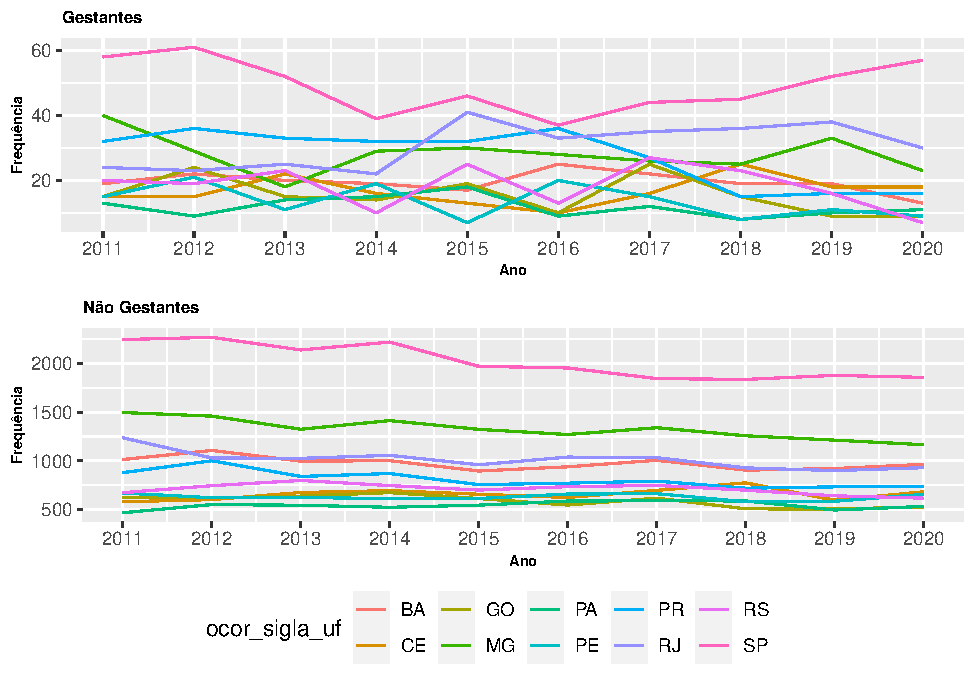
\includegraphics{RelatorioV01_files/figure-latex/unnamed-chunk-14-1.pdf}
\caption{Séries Temporáis por UF de Ocorrência}
\end{figure}

\hypertarget{teste-de-independuxeancia}{%
\section{Teste de Independência}\label{teste-de-independuxeancia}}

A análise da interferência das variáveis demográficas no número de
mortes de gestantes e não gestantes causadas por fatores externos é de
suma importância para compreender os possíveis determinantes desses
eventos de morte por fatores externos.

Para realizar essa análise, utilizaremos técnicas estatísticas, como o
teste qui-quadrado de independência que nos permitirá avaliar se as
variáveis demográficas estão associadas ao número de mortes em cada
grupo (gestantes e não gestantes). Caso sejam encontradas associações
significativas, será possível identificar quais variáveis demográficas
estão mais fortemente relacionadas com a mortalidade materna.

Como exposto anteriormente, a variável sexo não irá ser considerada,
devido a praticamente todos os dados (Dentro do esperado), serem de
mulheres.

\emph{CONVERSAR SOBRE ESSE TOPICO NA REUNIAO, NAO TEM COMO APLICAR O
TESTE QUI QUADRADO DEVIDO AO BAIXO NUMERO DE VALORES ESPERADOS PARA
ALGUMAS CATEGORIAS E O TESTE EXATO DE FISHER NAO E VALIDO, SURGIU A
SUGESTAO DE REGRESSAO BINOMIAL OU DESCONSIDERAR AS CATEGORIAS COM BAIXO
NUMERO DE OBSERVACOES}

\end{document}
